% Section~\ref{sec:mainstream_drl} outlined the theoretical taxonomy of DRL algorithms and their functional mechanisms in converter control. 
% Building on this theoretical foundation, the present section shifts focus from algorithmic structure to temporal evolution. 
% It examines how representative DRL algorithms have emerged, matured, and diversified over time, 
% tracing their adoption trajectories within PECs research. 
% The discussion highlights key historical milestones, characteristic application phases, 
% and emerging utilization trends revealed through recent literature statistics.


% \begin{figure*}[!t]
%   \centering
%   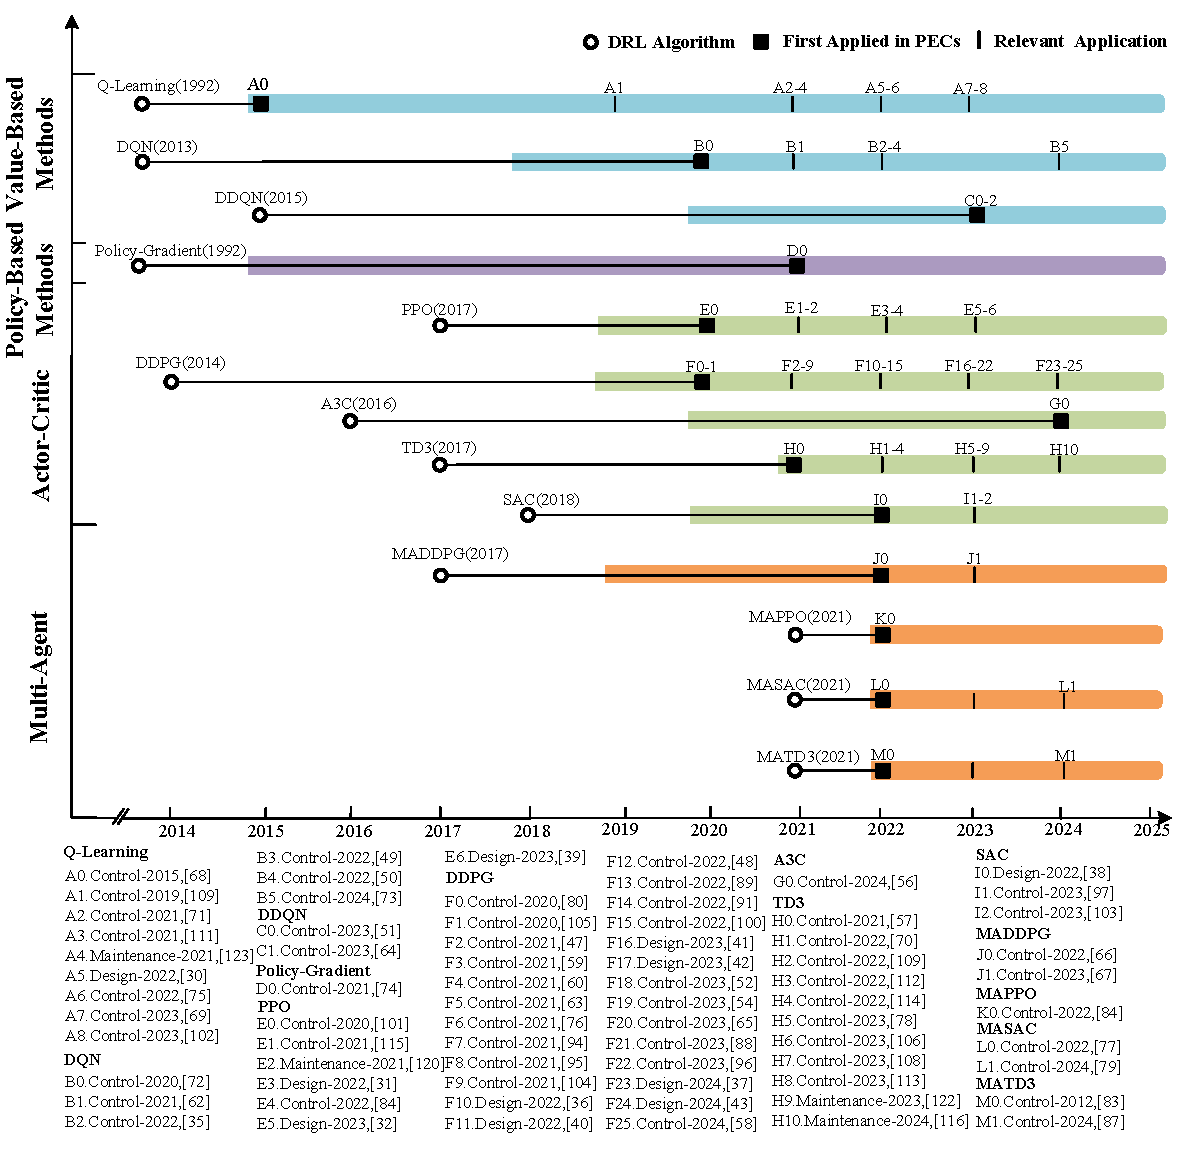
\includegraphics[width=0.9\textwidth]{fig/TIME_LINE5.pdf}
%   \caption{Timeline of representative DRL algorithms and their adoption in PECs.}
%   \label{fig:DRL_Timeline}
% \end{figure*} 

% Fig.~\ref{fig:DRL_Timeline} presents the chronological development and application milestones of representative DRL algorithms in PECs. The figure highlights the year each algorithm was introduced, its first reported adoption in PECs, and representative studies within each methodological category The information is based on the most widely recognized literature and is not exhaustive. Only algorithms that have demonstrated clear influence or potential in power-electronic applications are included for clarity.

% Several trends can be observed from Fig.~\ref{fig:DRL_Timeline} and Fig.\ref{fig:sunburst_tpel}. 

% 1) \textbf{Early stage—Value-based learning.}  
% The earliest applications of DRL in PECs, mainly between 2015 and 2017, relied on value-based algorithms such as Q-Learning, DQN, and DDQN. These methods offered interpretable decision processes and enabled discrete switching control through state–action mapping. Their simplicity made them suitable for initial proof-of-concept studies. However, they were inherently limited by discrete action definitions and slow convergence when applied to high-dimensional or continuous converter systems. As converter control increasingly required continuous and adaptive decision variables, the use of pure value-based methods gradually diminished.

% 2) \textbf{Intermediate stage—Policy-gradient optimization.}  
% The development of policy-gradient algorithms, including REINFORCE, TRPO, SVPG, and GRPO, marked the first step toward continuous control in DRL. These methods directly optimized the policy parameters without explicit value-function estimation, thereby enabling smooth and differentiable control actions such as duty-ratio or phase-shift regulation. Although conceptually elegant, policy-gradient methods exhibited high gradient variance and low sample efficiency, limiting their practical deployment in PECs. Consequently, they primarily served as theoretical precursors to the more stable actor–critic architectures.

% 3) \textbf{Mainstream stage—Actor–critic integration.}  
% From 2017 onward, actor–critic algorithms became the central framework for DRL applications in PECs. Representative methods such as DDPG, TD3, SAC, and PPO introduced various mechanisms to improve stability and convergence. DDPG extended deterministic control to continuous spaces but suffered from overestimation bias; TD3 mitigated this through twin critics and delayed target updates; SAC incorporated entropy regularization to balance exploration and exploitation; and PPO stabilized policy updates through clipped surrogate objectives. As illustrated in Fig.~\ref{fig:sunburst_tpel}, actor–critic methods collectively represent the majority of reported DRL applications in PECs, underscoring their adaptability to nonlinear, time-varying converter dynamics.

% 4) \textbf{Emerging stage—Multi-agent reinforcement learning.}  
% In recent years, multi-agent DRL (MADDPG, MAPPO, MASAC, MATD3) has emerged as a new frontier for distributed and cooperative converter control. These algorithms extend single-agent frameworks to multi-terminal or modular converter architectures through centralized training and decentralized execution. By enabling communication and coordination among agents, they support scalable control of interconnected systems such as microgrids, modular multilevel converters, and distributed energy interfaces. Despite higher computational and communication costs, multi-agent methods are increasingly explored for hierarchical and cooperative energy management.

% The distribution of DRL applications summarized in Fig.~\ref{fig:sunburst_tpel} further validates these observations. Actor–critic algorithms dominate the current literature, accounting for more than half of all studies, while value-based and policy-gradient approaches together represent approximately forty percent. Multi-agent extensions, although relatively new, already comprise nearly ten percent of published implementations, indicating a growing interest in distributed learning architectures for converter coordination.

% Table~\ref{tab:drltable} provides a concise summary of these algorithms, comparing their advantages, limitations, and representative PECs applications. Value-based methods remain effective for discrete and low-dimensional problems due to their interpretability and efficiency. Policy-gradient methods extend DRL to continuous control but require careful variance reduction and tuning. Actor–critic frameworks offer improved stability and sample utilization, forming the current mainstream of DRL-based converter research. Multi-agent extensions further expand scalability and robustness for future distributed converter networks.

% Overall, the chronological progression of DRL in PECs—from discrete value learning to continuous policy optimization, then to hybrid actor–critic integration and distributed multi-agent cooperation—reflects a consistent evolution toward greater adaptability, scalability, and autonomy. This evolution illustrates the growing convergence between algorithmic advances in artificial intelligence and the control demands of modern power electronics, paving the way for data-driven, adaptive, and resilient converter systems.

Section~\ref{sec:mainstream_drl} established the theoretical taxonomy and functional mechanisms of DRL algorithms used in converter control. 
Building on that foundation, this section shifts focus from algorithmic structure to temporal evolution, examining how representative DRL methods have emerged, matured, and diversified in PECs research. 
The discussion emphasizes key milestones, representative application phases, and utilization trends revealed through recent literature statistics.

Fig. \ref{fig:DRL_Timeline} illustrates the chronological evolution of DRL algorithms and their corresponding adoption in PECs. 
Each entry denotes the year the algorithm was introduced, its first reported application in converter-related studies, and representative works across the four principal families. 
For the sake of clarity, only algorithms with documented influence or significant potential in converter design, control and maintenance are included.  
% The data presented here were compiled from peer-reviewed publications indexed in IEEE Xplore and Google Scholar between 2015 and 2025, using the keywords ``deep reinforcement learning'' and ``power electronic converters.''\footnote{The quantitative statistics summarized in Fig.~\ref{fig:sunburst_tpel} and Table~\ref{tab:drltable} are based on 112 publications retrieved from IEEE Xplore and Google Scholar within this time window. Duplicate or derivative studies were excluded.}
% From Fig.~\ref{fig:DRL_Timeline} and Fig.~\ref{fig:sunburst_tpel}, several distinct evolutionary phases of DRL applications in PECs can be clearly discerned.



\begin{figure}[!t]
  \centering
  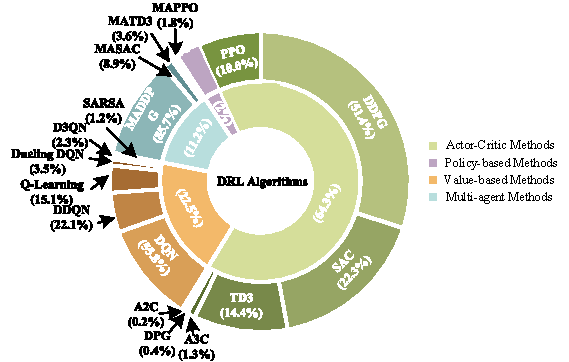
\includegraphics[width=\linewidth]{fig/pie_journal4.pdf}
  \caption{Application distribution of population-based DRL algorithms in PECs.}
  \label{fig:sunburst_tpel}
\end{figure}


\subsection{Early Stage: Value-Based Learning (2015--2017)}

During the early stage, DRL research in PECs primarily employed value-based algorithms such as Q-learning, DQN, and DDQN. 
These methods provided interpretable decision processes and enabled discrete switching control through explicit state--action mappings. 
Their simplicity made them well suited for proof-of-concept studies, including duty-cycle quantization, converter mode selection, and discrete-level buck or boost regulation
% ~\cite{10030117,9521987,schenke2021deep}.  
However, due to their reliance on discretized actions, they exhibited limited scalability and slow convergence when applied to high-dimensional or continuous converter dynamics. 
This stage established the feasibility of reinforcement-driven converter control but also exposed the need for smoother policy representations.

\subsection{Intermediate Stage: Policy-Gradient Optimization (2017--2019)}

The subsequent phase witnessed the emergence of policy-gradient algorithms, including REINFORCE, TRPO and SVPG, which directly optimized policy parameters without explicit value-function estimation.  
These methods facilitated differentiable and continuous control actions, enabling smoother duty-ratio and phase-shift regulation in converters such as single-phase inverters and resonant topologies
% ~\cite{jiang2021application}.  
Despite this advancement, policy-gradient approaches suffered from high variance in gradient estimation and low sample efficiency, which hindered real-time training.  
Their primary contribution lay in introducing continuous-action control to PECs, paving the way for hybrid frameworks that combine policy learning with value-based stabilization.

\subsection{Mainstream Stage: Actor--Critic Integration (2019--2023)}

From 2019 onward, AC algorithms became the predominant framework for DRL in PECs.  
Representative methods such as DDPG, TD3, SAC, and PPO achieved a balance between stability and adaptability through coordinated actor--critic updates.  
These methods were applied extensively to continuous converter control, including phase-shift optimization in dual-active-bridge (DAB) converters, adaptive droop control in microgrids, and harmonic suppression in grid-tied inverters
% ~\cite{10141314,ye2024deep,kosuru2022deep}. 
DDPG provided deterministic control for continuous tasks, TD3 improved critic stability via dual estimators, SAC enhanced exploration through entropy regularization, and PPO introduced clipped policy updates that ensured training robustness.  
As summarized in Fig.~\ref{fig:sunburst_tpel}, AC algorithms collectively account for more than half of all DRL-based converter studies, underscoring their robustness to nonlinearities, parameter drift, and unmodeled dynamics.


\begin{table*}[t]
\centering
\caption{Representative DRL Algorithms and Applications in PECs}
\label{tab:drltable}
\renewcommand{\arraystretch}{1.22}
\begin{tabular*}{\textwidth}{@{\extracolsep{\fill}} m{2cm} l p{5.0cm} p{5.2cm} p{3cm}@{}}
\toprule
\textbf{Category} & \textbf{Algorithm} & \textbf{Advantages} & \textbf{Limitations} & \textbf{Applications} \\
\midrule

\multirow{3}{*}{\textbf{Value-Based}}
& Q-Learning &
Simple structure;
Interpretable Q-table; Efficient in low-dimensional discrete tasks &
Discrete-only actions; 
Poor scalability;  Overestimation risk &
Design~[30]; \newline Control~[68,69,110,111]; \newline Maintenance~[123] \\ 
\cmidrule(l){2-5}

& DQN &
High-dimensional state representation; improved sample utility &
Large data demand; hyperparameter sensitivity; value overestimation &
Design~[35]; \newline Control~[49,50,72,73] \\ 
\cmidrule(l){2-5}

& DDQN &
Dual critics; reduced bias; stabilized convergence &
Higher computation; longer training &
Control~[51,64] \\
\midrule

\textbf{Policy-Based}
& Policy Gradient &
Direct policy optimization; continuous/discrete support; smooth adaptation &
High gradient variance; low sample efficiency; LR sensitivity &
Control~[74] \\
\midrule

\multirow{5}{*}{\textbf{Actor–Critic}}
& PPO &
Clipped updates; stable convergence; variance reduction &
Clip-ratio sensitivity; limited exploration &
Design~[31,32,39]; \newline Control~[84,101,115]; \newline Maintenance~[120] \\ 
\cmidrule(l){2-5}

& DDPG &
Deterministic policy; continuous control; high sample efficiency &
Noise sensitivity; reward-scaling dependence; divergence risk &
Design~[36,37,40]; \newline Control~[47,48,104,105] \\ 
\cmidrule(l){2-5}

& TD3 &
Twin critics; delayed updates; reduced bias &
Higher computation; multi-parameter coordination &
Control~[57,70,108,109]; \newline Maintenance~[116,122] \\ 
\cmidrule(l){2-5}

& SAC &
Entropy-regularized exploration; robustness under uncertainty &
High compute cost; slow convergence in deterministic tasks &
Design~[38]; \newline Control~[97,103] \\ 
\cmidrule(l){2-5}

& A3C &
Asynchronous training; enhanced exploration; fast learning &
Async instability; gradient noise &
Control~[56] \\
\midrule

\multirow{4}{*}{\textbf{Multi-Agent}}
& MADDPG &
Centralized training; decentralized execution; cooperative control &
Non-stationarity; communication dependence &
Control~[66,67] \\ 
\cmidrule(l){2-5}

& MAPPO &
Multi-agent PPO stability; scalable coordination &
Sync overhead; communication cost &
Control~[84] \\ 
\cmidrule(l){2-5}

& MASAC &
Entropy-driven exploration; robust cooperative behavior &
High computation; reward-coupling sensitivity &
Control~[77,79] \\ 
\cmidrule(l){2-5}

& MATD3 &
Twin critics for joint evaluation; improved multi-agent stability &
Bandwidth demand; implementation complexity &
Control~[83,87] \\
\bottomrule
\end{tabular*}
\end{table*}



\subsection{Emerging Stage: Multi-Agent Reinforcement Learning (2023--Present)}

Recent advances have expanded DRL from single-agent to multi-agent frameworks, introducing cooperative and distributed control paradigms for modular and large-scale PECs systems.  
Algorithms such as MADDPG, MAPPO, MASAC, and MATD3 have been adapted to enable centralized training with decentralized execution, promoting coordination among converter modules.  
Representative tasks include power-sharing control in interleaved series-output-parallel (ISOP) converters, arm-energy balancing in modular multilevel converters (MMCs), and distributed voltage regulation in microgrids.  
Although multi-agent methods introduce higher computational and communication costs, they provide scalability, resilience, and adaptive fault tolerance, marking a transition toward intelligent converter networks capable of cooperative decision-making.

\subsection{Lifecycle Extensions in Design and Maintenance (2021--Present)}

Beyond control-oriented implementations, DRL has begun to influence the design and maintenance stages of converter development.  
In the design phase, early studies employed value-based methods for discrete topology selection and passive component sizing
% ~\cite{9615058,tian2022deep}.  
More recent works have applied actor--critic frameworks for multi-objective optimization that balances efficiency, power density, and thermal performance
% ~\cite{wang2023efficiency,wang2024case}.  
In the maintenance domain, DRL has been explored for condition monitoring, anomaly detection, and predictive health management.  
Initial efforts used Q-learning or DQN for threshold-based fault identification
% ~\cite{huang2023reinforcement}, 
whereas newer studies have introduced TD3 and PPO agents for adaptive fault isolation and RUL prediction
% ~\cite{najafi2023deep,chen2024determining}.  
These advances indicate that the algorithmic progression observed in control applications is now extending to design optimization and health-aware operation, promoting a unified learning-driven lifecycle for intelligent PECs.

\subsection{Statistical Overview and Research Distribution}

The cumulative publication distribution in Fig.~\ref{fig:sunburst_tpel} reinforces these observations. 
AC methods dominate the literature, accounting for approximately 64.3\% of reported DRL-based PEC studies. 
Value-based algorithms represent about 22.5\%, policy-gradient methods about 2\%, and multi-agent frameworks roughly 11.2\%. 
This distribution demonstrates the prevailing preference for hybrid learning architectures while highlighting a gradual increase in cooperative and lifecycle-integrated approaches. 
Table~\ref{tab:drltable} summarizes the comparative advantages, limitations, and representative PECs tasks associated with each family.  
Value-based approaches provide interpretability and computational simplicity but are constrained by discretization.  
Policy-gradient methods enable continuous control yet require variance-reduction strategies.  
Actor--critic frameworks improve stability and sample utilization, while multi-agent algorithms extend scalability and system-level coordination.

\subsection{Discussion and Interpretation}

The chronological progression of DRL in PECs, from discrete value learning to continuous policy optimization, then to hybrid actor--critic integration and distributed multi-agent cooperation, 
reveals a consistent trend toward higher autonomy, scalability, and adaptability.  
This evolution also manifests beyond the control phase, as recent studies integrate DRL into converter design and predictive maintenance workflows.  
By bridging real-time control, design optimization, and health management, DRL is transforming converter research from model-dependent engineering to data-driven, self-optimizing, and resilient intelligent systems that operate seamlessly across the entire lifecycle of PECs.

